% Created by tikzDevice version 0.11 on 2018-06-14 22:19:05
% !TEX encoding = UTF-8 Unicode
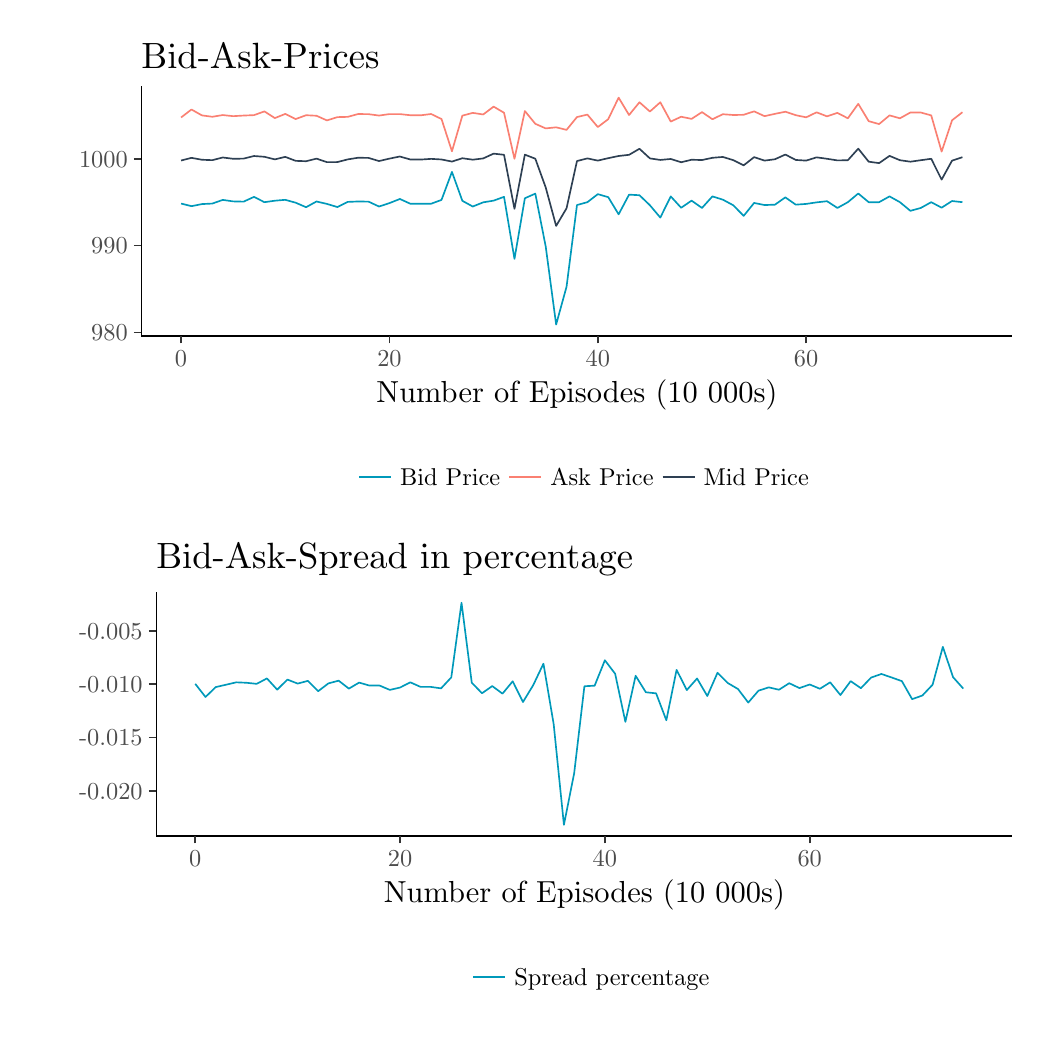
\begin{tikzpicture}[x=1pt,y=1pt]
\definecolor{fillColor}{RGB}{255,255,255}
\path[use as bounding box,fill=fillColor,fill opacity=0.00] (0,0) rectangle (361.35,361.35);
\begin{scope}
\path[clip] (  0.00,180.67) rectangle (361.35,361.35);
\definecolor{drawColor}{RGB}{255,255,255}
\definecolor{fillColor}{RGB}{255,255,255}

\path[draw=drawColor,line width= 0.6pt,line join=round,line cap=round,fill=fillColor] (  0.00,180.67) rectangle (361.35,361.35);
\end{scope}
\begin{scope}
\path[clip] ( 41.12,249.98) rectangle (355.85,340.16);
\definecolor{fillColor}{RGB}{255,255,255}

\path[fill=fillColor] ( 41.12,249.98) rectangle (355.85,340.16);
\definecolor{drawColor}{RGB}{0,153,186}

\path[draw=drawColor,line width= 0.6pt,line join=round] ( 55.43,297.79) --
	( 59.19,296.85) --
	( 62.96,297.60) --
	( 66.72,297.79) --
	( 70.49,299.11) --
	( 74.25,298.57) --
	( 78.02,298.48) --
	( 81.78,300.20) --
	( 85.55,298.29) --
	( 89.31,298.82) --
	( 93.07,299.14) --
	( 96.84,298.10) --
	(100.60,296.47) --
	(104.37,298.54) --
	(108.13,297.66) --
	(111.90,296.53) --
	(115.66,298.39) --
	(119.43,298.54) --
	(123.19,298.48) --
	(126.96,296.72) --
	(130.72,297.95) --
	(134.49,299.45) --
	(138.25,297.73) --
	(142.02,297.70) --
	(145.78,297.73) --
	(149.54,299.11) --
	(153.31,309.23) --
	(157.07,298.78) --
	(160.84,296.72) --
	(164.60,298.23) --
	(168.37,298.85) --
	(172.13,300.22) --
	(175.90,277.79) --
	(179.66,299.71) --
	(183.43,301.38) --
	(187.19,282.28) --
	(190.96,254.08) --
	(194.72,267.74) --
	(198.49,297.25) --
	(202.25,298.29) --
	(206.02,301.19) --
	(209.78,300.10) --
	(213.54,293.90) --
	(217.31,301.01) --
	(221.07,300.80) --
	(224.84,297.18) --
	(228.60,292.72) --
	(232.37,300.38) --
	(236.13,296.27) --
	(239.90,298.85) --
	(243.66,296.20) --
	(247.43,300.38) --
	(251.19,299.20) --
	(254.96,297.18) --
	(258.72,293.34) --
	(262.49,298.01) --
	(266.25,297.25) --
	(270.02,297.39) --
	(273.78,300.03) --
	(277.54,297.39) --
	(281.31,297.66) --
	(285.07,298.22) --
	(288.84,298.64) --
	(292.60,296.20) --
	(296.37,298.29) --
	(300.13,301.43) --
	(303.90,298.29) --
	(307.66,298.29) --
	(311.43,300.38) --
	(315.19,298.29) --
	(318.96,295.16) --
	(322.72,296.20) --
	(326.49,298.29) --
	(330.25,296.30) --
	(334.01,298.71) --
	(337.78,298.29);
\definecolor{drawColor}{RGB}{250,128,114}

\path[draw=drawColor,line width= 0.6pt,line join=round] ( 55.43,328.90) --
	( 59.19,331.78) --
	( 62.96,329.65) --
	( 66.72,329.15) --
	( 70.49,329.77) --
	( 74.25,329.37) --
	( 78.02,329.59) --
	( 81.78,329.74) --
	( 85.55,331.09) --
	( 89.31,328.68) --
	( 93.07,330.18) --
	( 96.84,328.33) --
	(100.60,329.71) --
	(104.37,329.52) --
	(108.13,327.83) --
	(111.90,329.02) --
	(115.66,329.12) --
	(119.43,330.15) --
	(123.19,330.09) --
	(126.96,329.59) --
	(130.72,330.12) --
	(134.49,330.12) --
	(138.25,329.71) --
	(142.02,329.68) --
	(145.78,330.15) --
	(149.54,328.33) --
	(153.31,316.68) --
	(157.07,329.55) --
	(160.84,330.56) --
	(164.60,329.98) --
	(168.37,332.82) --
	(172.13,330.60) --
	(175.90,313.97) --
	(179.66,331.22) --
	(183.43,326.61) --
	(187.19,324.95) --
	(190.96,325.34) --
	(194.72,324.42) --
	(198.49,329.05) --
	(202.25,329.93) --
	(206.02,325.43) --
	(209.78,328.28) --
	(213.54,336.06) --
	(217.31,329.79) --
	(221.07,334.39) --
	(224.84,331.04) --
	(228.60,334.39) --
	(232.37,327.42) --
	(236.13,329.16) --
	(239.90,328.39) --
	(243.66,330.83) --
	(247.43,328.26) --
	(251.19,330.07) --
	(254.96,329.79) --
	(258.72,329.86) --
	(262.49,331.11) --
	(266.25,329.37) --
	(270.02,330.21) --
	(273.78,330.97) --
	(277.54,329.72) --
	(281.31,328.95) --
	(285.07,330.76) --
	(288.84,329.30) --
	(292.60,330.55) --
	(296.37,328.60) --
	(300.13,333.83) --
	(303.90,327.56) --
	(307.66,326.51) --
	(311.43,329.65) --
	(315.19,328.60) --
	(318.96,330.69) --
	(322.72,330.69) --
	(326.49,329.65) --
	(330.25,316.58) --
	(334.01,327.87) --
	(337.78,330.80);
\definecolor{drawColor}{RGB}{46,64,83}

\path[draw=drawColor,line width= 0.6pt,line join=round] ( 55.43,313.34) --
	( 59.19,314.31) --
	( 62.96,313.62) --
	( 66.72,313.47) --
	( 70.49,314.44) --
	( 74.25,313.97) --
	( 78.02,314.03) --
	( 81.78,314.97) --
	( 85.55,314.69) --
	( 89.31,313.75) --
	( 93.07,314.66) --
	( 96.84,313.22) --
	(100.60,313.09) --
	(104.37,314.03) --
	(108.13,312.75) --
	(111.90,312.78) --
	(115.66,313.75) --
	(119.43,314.35) --
	(123.19,314.28) --
	(126.96,313.15) --
	(130.72,314.03) --
	(134.49,314.79) --
	(138.25,313.72) --
	(142.02,313.69) --
	(145.78,313.94) --
	(149.54,313.72) --
	(153.31,312.96) --
	(157.07,314.17) --
	(160.84,313.64) --
	(164.60,314.10) --
	(168.37,315.83) --
	(172.13,315.41) --
	(175.90,295.88) --
	(179.66,315.46) --
	(183.43,314.00) --
	(187.19,303.61) --
	(190.96,289.71) --
	(194.72,296.08) --
	(198.49,313.15) --
	(202.25,314.11) --
	(206.02,313.31) --
	(209.78,314.19) --
	(213.54,314.98) --
	(217.31,315.40) --
	(221.07,317.59) --
	(224.84,314.11) --
	(228.60,313.55) --
	(232.37,313.90) --
	(236.13,312.72) --
	(239.90,313.62) --
	(243.66,313.52) --
	(247.43,314.32) --
	(251.19,314.63) --
	(254.96,313.48) --
	(258.72,311.60) --
	(262.49,314.56) --
	(266.25,313.31) --
	(270.02,313.80) --
	(273.78,315.50) --
	(277.54,313.55) --
	(281.31,313.31) --
	(285.07,314.49) --
	(288.84,313.97) --
	(292.60,313.38) --
	(296.37,313.45) --
	(300.13,317.63) --
	(303.90,312.92) --
	(307.66,312.40) --
	(311.43,315.02) --
	(315.19,313.45) --
	(318.96,312.92) --
	(322.72,313.45) --
	(326.49,313.97) --
	(330.25,306.44) --
	(334.01,313.29) --
	(337.78,314.54);
\end{scope}
\begin{scope}
\path[clip] (  0.00,  0.00) rectangle (361.35,361.35);
\definecolor{drawColor}{RGB}{0,0,0}

\path[draw=drawColor,line width= 0.6pt,line join=round] ( 41.12,249.98) --
	( 41.12,340.16);
\end{scope}
\begin{scope}
\path[clip] (  0.00,  0.00) rectangle (361.35,361.35);
\definecolor{drawColor}{gray}{0.30}

\node[text=drawColor,anchor=base east,inner sep=0pt, outer sep=0pt, scale=  0.88] at ( 36.17,248.22) {980};

\node[text=drawColor,anchor=base east,inner sep=0pt, outer sep=0pt, scale=  0.88] at ( 36.17,279.58) {990};

\node[text=drawColor,anchor=base east,inner sep=0pt, outer sep=0pt, scale=  0.88] at ( 36.17,310.94) {1000};
\end{scope}
\begin{scope}
\path[clip] (  0.00,  0.00) rectangle (361.35,361.35);
\definecolor{drawColor}{gray}{0.20}

\path[draw=drawColor,line width= 0.6pt,line join=round] ( 38.37,251.25) --
	( 41.12,251.25);

\path[draw=drawColor,line width= 0.6pt,line join=round] ( 38.37,282.61) --
	( 41.12,282.61);

\path[draw=drawColor,line width= 0.6pt,line join=round] ( 38.37,313.97) --
	( 41.12,313.97);
\end{scope}
\begin{scope}
\path[clip] (  0.00,  0.00) rectangle (361.35,361.35);
\definecolor{drawColor}{RGB}{0,0,0}

\path[draw=drawColor,line width= 0.6pt,line join=round] ( 41.12,249.98) --
	(355.85,249.98);
\end{scope}
\begin{scope}
\path[clip] (  0.00,  0.00) rectangle (361.35,361.35);
\definecolor{drawColor}{gray}{0.20}

\path[draw=drawColor,line width= 0.6pt,line join=round] ( 55.43,247.23) --
	( 55.43,249.98);

\path[draw=drawColor,line width= 0.6pt,line join=round] (130.72,247.23) --
	(130.72,249.98);

\path[draw=drawColor,line width= 0.6pt,line join=round] (206.02,247.23) --
	(206.02,249.98);

\path[draw=drawColor,line width= 0.6pt,line join=round] (281.31,247.23) --
	(281.31,249.98);
\end{scope}
\begin{scope}
\path[clip] (  0.00,  0.00) rectangle (361.35,361.35);
\definecolor{drawColor}{gray}{0.30}

\node[text=drawColor,anchor=base,inner sep=0pt, outer sep=0pt, scale=  0.88] at ( 55.43,238.97) {0};

\node[text=drawColor,anchor=base,inner sep=0pt, outer sep=0pt, scale=  0.88] at (130.72,238.97) {20};

\node[text=drawColor,anchor=base,inner sep=0pt, outer sep=0pt, scale=  0.88] at (206.02,238.97) {40};

\node[text=drawColor,anchor=base,inner sep=0pt, outer sep=0pt, scale=  0.88] at (281.31,238.97) {60};
\end{scope}
\begin{scope}
\path[clip] (  0.00,  0.00) rectangle (361.35,361.35);
\definecolor{drawColor}{RGB}{0,0,0}

\node[text=drawColor,anchor=base,inner sep=0pt, outer sep=0pt, scale=  1.10] at (198.49,225.89) {Number of Episodes (10 000s)};
\end{scope}
\begin{scope}
\path[clip] (  0.00,  0.00) rectangle (361.35,361.35);
\definecolor{fillColor}{RGB}{255,255,255}

\path[fill=fillColor] (109.01,186.17) rectangle (287.96,212.01);
\end{scope}
\begin{scope}
\path[clip] (  0.00,  0.00) rectangle (361.35,361.35);
\definecolor{drawColor}{RGB}{0,153,186}

\path[draw=drawColor,line width= 0.6pt,line join=round] (119.76,199.09) -- (131.32,199.09);
\end{scope}
\begin{scope}
\path[clip] (  0.00,  0.00) rectangle (361.35,361.35);
\definecolor{drawColor}{RGB}{250,128,114}

\path[draw=drawColor,line width= 0.6pt,line join=round] (174.02,199.09) -- (185.58,199.09);
\end{scope}
\begin{scope}
\path[clip] (  0.00,  0.00) rectangle (361.35,361.35);
\definecolor{drawColor}{RGB}{46,64,83}

\path[draw=drawColor,line width= 0.6pt,line join=round] (229.43,199.09) -- (240.99,199.09);
\end{scope}
\begin{scope}
\path[clip] (  0.00,  0.00) rectangle (361.35,361.35);
\definecolor{drawColor}{RGB}{0,0,0}

\node[text=drawColor,anchor=base west,inner sep=0pt, outer sep=0pt, scale=  0.88] at (134.57,196.06) {Bid Price};
\end{scope}
\begin{scope}
\path[clip] (  0.00,  0.00) rectangle (361.35,361.35);
\definecolor{drawColor}{RGB}{0,0,0}

\node[text=drawColor,anchor=base west,inner sep=0pt, outer sep=0pt, scale=  0.88] at (188.84,196.06) {Ask Price};
\end{scope}
\begin{scope}
\path[clip] (  0.00,  0.00) rectangle (361.35,361.35);
\definecolor{drawColor}{RGB}{0,0,0}

\node[text=drawColor,anchor=base west,inner sep=0pt, outer sep=0pt, scale=  0.88] at (244.25,196.06) {Mid Price};
\end{scope}
\begin{scope}
\path[clip] (  0.00,  0.00) rectangle (361.35,361.35);
\definecolor{drawColor}{RGB}{0,0,0}

\node[text=drawColor,anchor=base west,inner sep=0pt, outer sep=0pt, scale=  1.32] at ( 41.12,346.76) {Bid-Ask-Prices};
\end{scope}
\begin{scope}
\path[clip] (  0.00,  0.00) rectangle (361.35,180.67);
\definecolor{drawColor}{RGB}{255,255,255}
\definecolor{fillColor}{RGB}{255,255,255}

\path[draw=drawColor,line width= 0.6pt,line join=round,line cap=round,fill=fillColor] (  0.00, -0.00) rectangle (361.35,180.67);
\end{scope}
\begin{scope}
\path[clip] ( 46.50, 69.30) rectangle (355.85,157.54);
\definecolor{fillColor}{RGB}{255,255,255}

\path[fill=fillColor] ( 46.50, 69.30) rectangle (355.85,157.54);
\definecolor{drawColor}{RGB}{0,153,186}

\path[draw=drawColor,line width= 0.6pt,line join=round] ( 60.56,124.23) --
	( 64.26,119.49) --
	( 67.96,123.07) --
	( 71.66,123.92) --
	( 75.36,124.79) --
	( 79.06,124.63) --
	( 82.76,124.24) --
	( 86.46,126.20) --
	( 90.16,122.14) --
	( 93.86,125.79) --
	( 97.56,124.33) --
	(101.26,125.32) --
	(104.96,121.58) --
	(108.66,124.40) --
	(112.37,125.39) --
	(116.07,122.51) --
	(119.77,124.70) --
	(123.47,123.62) --
	(127.17,123.62) --
	(130.87,122.05) --
	(134.57,122.91) --
	(138.27,124.79) --
	(141.97,123.14) --
	(145.67,123.14) --
	(149.37,122.60) --
	(153.07,126.57) --
	(156.77,153.53) --
	(160.47,124.66) --
	(164.17,120.84) --
	(167.87,123.44) --
	(171.57,120.70) --
	(175.27,125.16) --
	(178.97,117.67) --
	(182.67,123.76) --
	(186.37,131.53) --
	(190.07,109.67) --
	(193.77, 73.31) --
	(197.47, 91.91) --
	(201.17,123.37) --
	(204.87,123.58) --
	(208.57,132.76) --
	(212.28,127.88) --
	(215.98,110.50) --
	(219.68,127.15) --
	(223.38,121.20) --
	(227.08,120.81) --
	(230.78,111.08) --
	(234.48,129.29) --
	(238.18,122.00) --
	(241.88,126.17) --
	(245.58,119.85) --
	(249.28,128.26) --
	(252.98,124.54) --
	(256.68,122.36) --
	(260.38,117.48) --
	(264.08,121.77) --
	(267.78,122.97) --
	(271.48,122.11) --
	(275.18,124.47) --
	(278.88,122.71) --
	(282.58,124.01) --
	(286.28,122.46) --
	(289.98,124.79) --
	(293.68,120.19) --
	(297.38,125.22) --
	(301.08,122.67) --
	(304.78,126.51) --
	(308.49,127.81) --
	(312.19,126.54) --
	(315.89,125.22) --
	(319.59,118.71) --
	(323.29,120.02) --
	(326.99,123.93) --
	(330.69,137.61) --
	(334.39,126.65) --
	(338.09,122.51);
\end{scope}
\begin{scope}
\path[clip] (  0.00,  0.00) rectangle (361.35,361.35);
\definecolor{drawColor}{RGB}{0,0,0}

\path[draw=drawColor,line width= 0.6pt,line join=round] ( 46.50, 69.30) --
	( 46.50,157.54);
\end{scope}
\begin{scope}
\path[clip] (  0.00,  0.00) rectangle (361.35,361.35);
\definecolor{drawColor}{gray}{0.30}

\node[text=drawColor,anchor=base east,inner sep=0pt, outer sep=0pt, scale=  0.88] at ( 41.55, 82.50) {-0.020};

\node[text=drawColor,anchor=base east,inner sep=0pt, outer sep=0pt, scale=  0.88] at ( 41.55,101.80) {-0.015};

\node[text=drawColor,anchor=base east,inner sep=0pt, outer sep=0pt, scale=  0.88] at ( 41.55,121.09) {-0.010};

\node[text=drawColor,anchor=base east,inner sep=0pt, outer sep=0pt, scale=  0.88] at ( 41.55,140.38) {-0.005};
\end{scope}
\begin{scope}
\path[clip] (  0.00,  0.00) rectangle (361.35,361.35);
\definecolor{drawColor}{gray}{0.20}

\path[draw=drawColor,line width= 0.6pt,line join=round] ( 43.75, 85.54) --
	( 46.50, 85.54);

\path[draw=drawColor,line width= 0.6pt,line join=round] ( 43.75,104.83) --
	( 46.50,104.83);

\path[draw=drawColor,line width= 0.6pt,line join=round] ( 43.75,124.12) --
	( 46.50,124.12);

\path[draw=drawColor,line width= 0.6pt,line join=round] ( 43.75,143.41) --
	( 46.50,143.41);
\end{scope}
\begin{scope}
\path[clip] (  0.00,  0.00) rectangle (361.35,361.35);
\definecolor{drawColor}{RGB}{0,0,0}

\path[draw=drawColor,line width= 0.6pt,line join=round] ( 46.50, 69.30) --
	(355.85, 69.30);
\end{scope}
\begin{scope}
\path[clip] (  0.00,  0.00) rectangle (361.35,361.35);
\definecolor{drawColor}{gray}{0.20}

\path[draw=drawColor,line width= 0.6pt,line join=round] ( 60.56, 66.55) --
	( 60.56, 69.30);

\path[draw=drawColor,line width= 0.6pt,line join=round] (134.57, 66.55) --
	(134.57, 69.30);

\path[draw=drawColor,line width= 0.6pt,line join=round] (208.57, 66.55) --
	(208.57, 69.30);

\path[draw=drawColor,line width= 0.6pt,line join=round] (282.58, 66.55) --
	(282.58, 69.30);
\end{scope}
\begin{scope}
\path[clip] (  0.00,  0.00) rectangle (361.35,361.35);
\definecolor{drawColor}{gray}{0.30}

\node[text=drawColor,anchor=base,inner sep=0pt, outer sep=0pt, scale=  0.88] at ( 60.56, 58.29) {0};

\node[text=drawColor,anchor=base,inner sep=0pt, outer sep=0pt, scale=  0.88] at (134.57, 58.29) {20};

\node[text=drawColor,anchor=base,inner sep=0pt, outer sep=0pt, scale=  0.88] at (208.57, 58.29) {40};

\node[text=drawColor,anchor=base,inner sep=0pt, outer sep=0pt, scale=  0.88] at (282.58, 58.29) {60};
\end{scope}
\begin{scope}
\path[clip] (  0.00,  0.00) rectangle (361.35,361.35);
\definecolor{drawColor}{RGB}{0,0,0}

\node[text=drawColor,anchor=base,inner sep=0pt, outer sep=0pt, scale=  1.10] at (201.17, 45.22) {Number of Episodes (10 000s)};
\end{scope}
\begin{scope}
\path[clip] (  0.00,  0.00) rectangle (361.35,361.35);
\definecolor{fillColor}{RGB}{255,255,255}

\path[fill=fillColor] (150.33,  5.50) rectangle (252.02, 31.34);
\end{scope}
\begin{scope}
\path[clip] (  0.00,  0.00) rectangle (361.35,361.35);
\definecolor{drawColor}{RGB}{0,153,186}

\path[draw=drawColor,line width= 0.6pt,line join=round] (161.08, 18.42) -- (172.64, 18.42);
\end{scope}
\begin{scope}
\path[clip] (  0.00,  0.00) rectangle (361.35,361.35);
\definecolor{drawColor}{RGB}{0,0,0}

\node[text=drawColor,anchor=base west,inner sep=0pt, outer sep=0pt, scale=  0.88] at (175.90, 15.39) {Spread percentage};
\end{scope}
\begin{scope}
\path[clip] (  0.00,  0.00) rectangle (361.35,361.35);
\definecolor{drawColor}{RGB}{0,0,0}

\node[text=drawColor,anchor=base west,inner sep=0pt, outer sep=0pt, scale=  1.32] at ( 46.50,166.08) {Bid-Ask-Spread in percentage};
\end{scope}
\end{tikzpicture}
